\chapter{边缘智能裂缝检测系统设计与实现}
本章基于第三章提出的裂缝检测算法,设计和实现边缘智能裂缝检测系统,并基于该边缘系统进行系统推理时延和功能测试的相关实验和结果分析。

%————————————————————————————————————————————边缘设备平台—————————————————————————————————————————————————————————————————————————
\section{边缘芯片平台}
本文算法部署和实验采用的边缘设备平台是海思Taurus套件。
该套件采用的芯片是海思Hi3516DV300。

\subsection{芯片及外设参数}

(1)核心处理器为双核ARM Cortex-A7处理器,工作频率为达900MHz,配备32KB I-Cache和32KB D-Cache,以及256KB的L2缓存,支持Neon加速和浮点运算单元(FPU),用于视频分析和智能计算及其调度。

(2)集成图像信号处理器ISP,用于图像质量优化和色彩处理。

(3)采用H.265视频压缩编码器。

(4)摄像头采用的是索尼高端安防低照度Sensor IMX335。

\subsection{智能计算平台}
Hi3516DV300芯片的智能计算平台由NNIE和IVE两部分组成。

其中,NNIE(Neural Network Inference Engine),是专门用于卷积神经网络推理的加速器,其算力为1.0TOPS。在本文模型部署中用于裂缝检测模型的推理运算。
IVE(Intelligent Video Engine),用于传统计算机视觉算法处理的加速引擎,
主要用于卷积神经网络算法的预处理及后处理上。在本文模型部署中用于对采集的裂缝帧/图像进行色彩空间转换、缩放、剪切等操作。

\subsection{芯片架构}
Hi3516DV300芯片由CPU子系统、视频子系统、图像子系统、AI子系统以及总线外设等部分组成,其芯片架构图见下图所示:

\begin{figure}[H]
    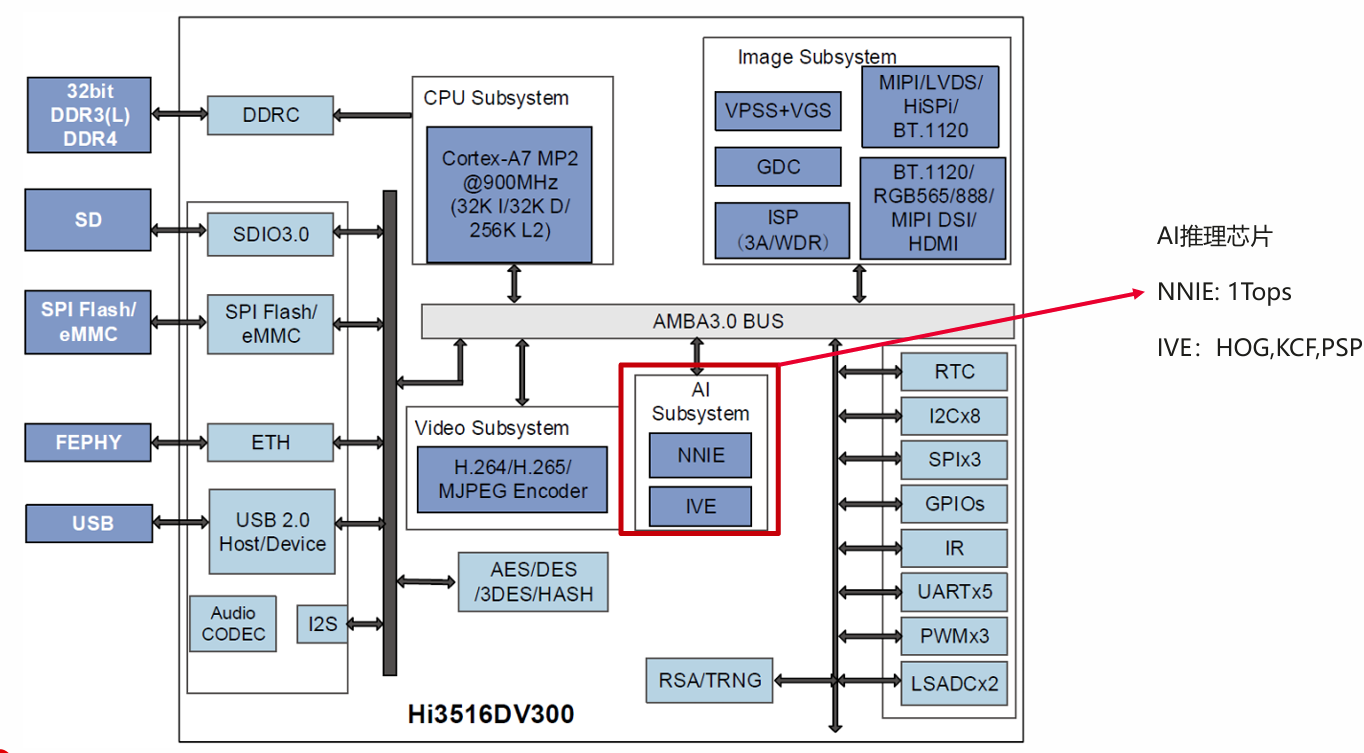
\includegraphics[width=14cm, height=8cm]{pic/Hi3516DV300-architect.png}      
    \label{hi3516dv300-architect}
    \caption{Hi3516DV300芯片架构图}
\end{figure}

Hi3516DV300设备实物图,如下图所示:
\begin{figure}[H]
    \subfloat[]{
        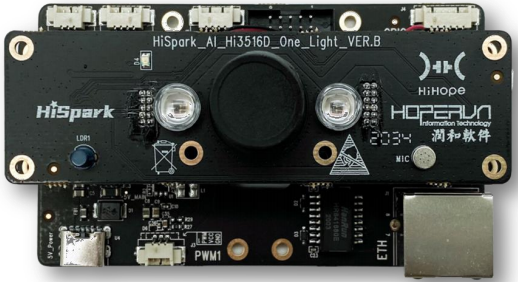
\includegraphics[width=7cm, height=4cm]{pic/taurus.png}       
        \label{taurus}
    }
    \subfloat[]{
        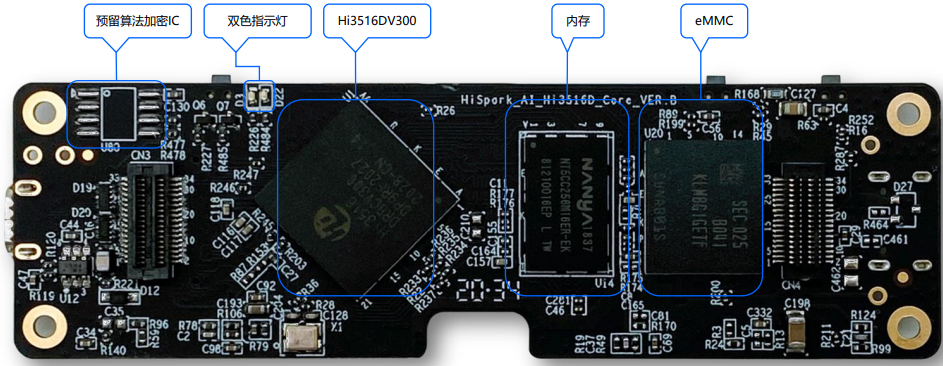
\includegraphics[width=7cm, height=4cm]{pic/Hi3516dv00.png}
        \label{hi3516dv300}
    }
    \caption{taurus套件与Hi3516DV300芯片}
    \label{taurus-hi3516dv300}
\end{figure}    

该芯片平台功耗低、资源有限、成本低,对于实际产业应用,更具备可行性,因此本文采用该平台作为部署和实验的边缘设备平台。




%————————————————————————————————————————————环境配置—————————————————————————————————————————————————————————————————————————
\section{环境配置}
海思Hi3516DV300芯片平台的环境配置,主要是编译和烧录基于Linux内核的OpenHarmony小型操作系统。

\subsection{系统编译}
系统编译指的是基于PC端的x86平台和Ubuntu20.04系统环境,将linux内核OpenHarmony小型操作系统,交叉编译为适配于Hi3516DV300芯片ARM平台的系统镜像。

\textbf{(1)OpenHarmony源码下载}

OpenHarmony是一项由开放原子基金会维护的开源操作系统项目,该操作系统旨在打造面向万物时代的全场景、微内核操作系统。
该操作系统最大特点在于内核可裁剪,可根据不同边缘设备的资源大小,灵活裁剪内核,实现全场景、高效的系统建构。

本文HI3516DV300芯片平台采用的操作系统是OpenHarmony的小型系统,内核为linux内核。该系统的主干源码下载及其详细介绍可在https://gitee.com/openharmony获取。

\textbf{(2)OpenHarmony源码编译}

首先,需要在PC端Ubuntu20.04系统中,安装编译OpenHarmony所需的库和工具,包括Python3.8、Java8、arm-linux-gnueabihf-gcc交叉编译链等工具和库。

其次,在OpenHarmony源码根目录下,安装编译OpenHarmony专用的编译工具hb(OpenHarmony编译子系统以GN和Ninjia构建为基座),
用于整编输出对应特定平台的系统镜像。

最后,设置编译路径,输入命令hb set,并选择对应平台ipcamera\_hispark\_taurus,然后进行系统编译,系统编译过程如下图所示:
\begin{figure}[H]
    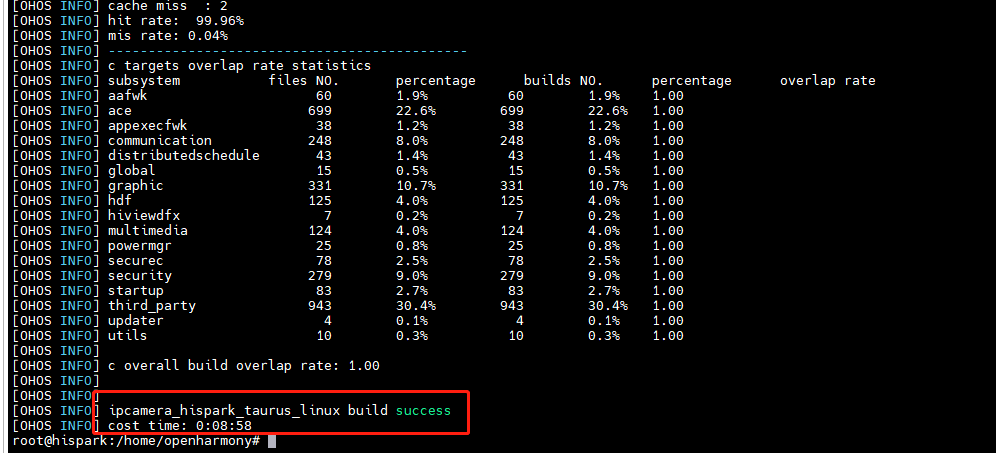
\includegraphics[width=12cm, height=7cm]{pic/build-taurus.png}
    \caption{Hi3516Dv300系统编译成功示意图}
    \label{build-taurus}
\end{figure}

系统交叉编译成功后,会在在out/hispark\_taurus/ipcamera\_hispark\_taurus\_linux目录下生成四个镜像文件,
分别是rootfs\_ext4.img, uImage\_hi3516dv300\_smp, userdata\_ext4.img ,userfs\_ext4.img。

\subsection{系统烧录}
系统烧录指的是基于PC端windows平台,使用USB通信方式和专用的烧录工具,将编译好的OpenHarmony小型系统镜像,烧录至Hi3516DV300芯片的Flash存储器中,并进行系统初始化。

\textbf{(1)串口驱动安装}

用户需要基于串口UART,实现PC端与海思3516DV300芯片平台之间的通信,用于系统初始化和后续应用程序加载。

下载和安装USB转串口驱动CH340,安装成功,可在PC段设备管理器查看端口,示意图如下:
\begin{figure}
    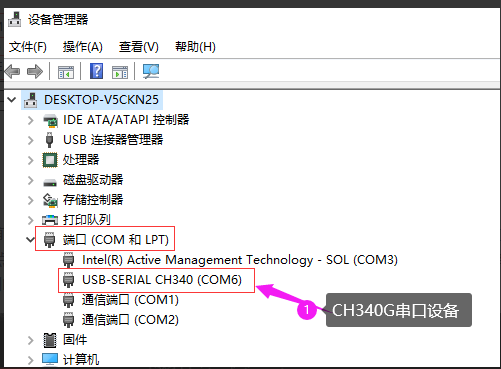
\includegraphics[width=12cm, height=8cm]{pic/usb-serial-340.png}
    \caption{串口驱动安装成功示意图}
    \label{usb-serial-ch340}
\end{figure}

\textbf{(2)烧录工具安装}

首先,安装USB驱动,本节系统烧录时,PC端与海思3516平台通信方式为USB通信,USB烧录相比串口烧录,数据通信速率更高、更稳定。

然后,下载和安装HiTool烧录工具,这是一款专门用于海思芯片系统烧录的工具。

\textbf{(3)系统烧录与初始化}

首先,在HiTool工具根目录下新建Images文件夹,并将rootfs\_ext4.img、uImage\_hi3516dv300\_smp、userdata\_ext4.img、userfs\_ext4.img编译得到的四个
镜像文件,以及源码/hi3516dv300/uboot/目录下的u-boot-hi3516dv300\_emmc.bin、partition.xml两个uboot启动引导和分区文件复制到Images目录下,
接着使用HiTool工具开始系统烧录。

然后,在系统烧录完成后,使用串口与芯片端进行通信,依次输入启动参数评率,完成系统初始化。如下图所示:

\begin{figure}[H]
    \subfloat[]{
        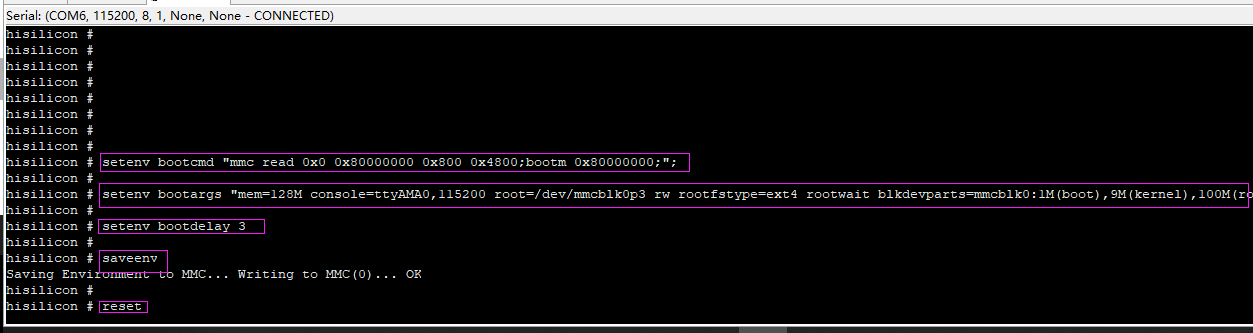
\includegraphics[width=7cm, height=5cm]{pic/cmd.png}      
        \label{cmd}
    }
    \subfloat[]{
        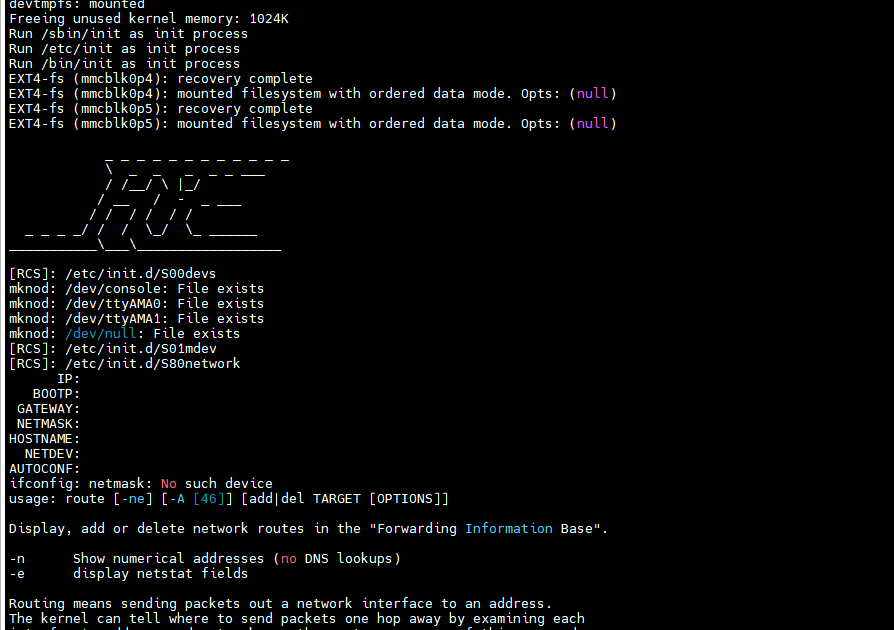
\includegraphics[width=7cm, height=5cm]{pic/success.png}
        \label{success}
    }
    \caption{系统初始化示意图}
    \label{taurus-init}
\end{figure}  

\subsection{系统测试}
系统烧录完成,编写Hello World程序,实现从视频采集、视频处理、视频显示全码流运行,系统测试成功效果,如下图所示:
\begin{figure}[H]
    \subfloat[]{
        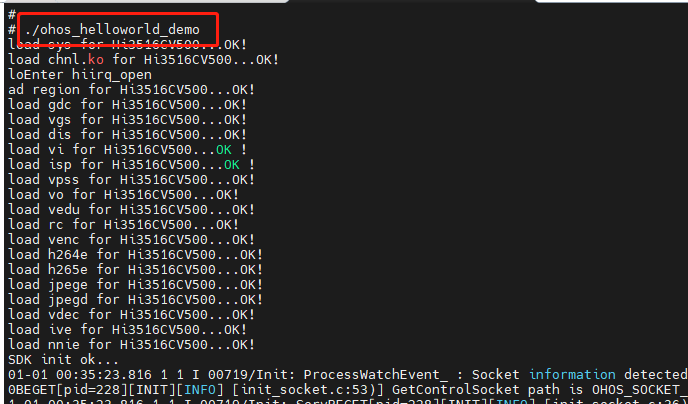
\includegraphics[width=7cm, height=5cm]{pic/test1.png}     
        \label{test1}
    }
    \subfloat[]{
        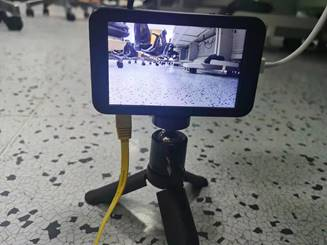
\includegraphics[width=7cm, height=5cm]{pic/test2.jpg}
        \label{test2}
    }
    \caption{系统初始化示意图}
    \label{system-test}
\end{figure}  



%————————————————————————————————————————————模型量化与部署—————————————————————————————————————————————————————————————————————————
\section{模型部署}
在前文中,已经介绍了边缘芯片平台及其芯片环境配置。
本节将详细介绍基于海思3516DV300边缘芯片平台,部署模型,实现对裂缝的实时视频检测。
主要由模型转换、模型量化和模型推理三个步骤组成。

\subsection{模型转换}
由于海思Hi3516DV300的NNIE AI加速器仅支持编译基于Caffe框架的模型,而本文模型是基于PyTorch框架进行编写实现,
故需要在模型部署前,进行模型框架转换,以适配NNIE加速器。

本文基于torch2caffe开源项目,进行模型框架转换,将model.pth文件转换为model.caffemodel和model.prototxt文件。
其中,model.caffemodel文件保存了基于Caffe框架的模型权重和偏置参数。model.prototxt文件则是对模型数据流和模型结构的描述性文本文件。

\subsection{模型量化}
为了提高模型在端侧推理的速度和实时性,模型量化成为端侧模型部署的一项重要技术。

模型量化指的是将机器学习模型的参数和计算从高精度表示(如32位浮点数)转换为低精度表示(如8位整数)的过程。
该技术有利于进一步减少模型大小,降低模型存储需求,缩小模型计算资源的需求,从而减少能耗,加速模型推理时延。

常见的量化方法包括线性量化和对数量化。

\textbf{(1)线性量化}

假设有一个浮点数向量$X = [x_1,x_2,x_3,...,x_N]$,
首先确定浮点数范围:
\begin{align}
    max(x) &= max(x_1,x_2,x_3,...,x_N) \\
    min(x) &= min(x_1,x_2,x_3,...,x_N) 
\end{align}

其次,定义量化步长$\Delta$,对于线性量化,步长为:
\begin{equation}
    \Delta = \frac{max(x)-min(x)}{2^n - 1}
\end{equation}

上式中,$2^n$表示量化级别的数量,$n$表示量化位数。

最后,将浮点数$x$映射到量化后的整数$q$:
\begin{equation}
    q = round(\frac{x-min(x)}{\Delta})
\end{equation}

其中,$round$表示四舍五入,这样一个浮点数将会量化为一个整数,该整数取值范围为$[0,2^n-1]$。

\textbf{(2)对数量化}

对数量化与线性量化类似,只是修改量化映射方式取对数映射:
\begin{equation}
    \Delta = \frac{log(max(x))-log(min(x))}{2^n - 1}
\end{equation}

模型量化尽管有利于减少存储和计算量、加速模型推理,但是也存在一定的精度损失,需要在实际应用中加以权衡和实验。

本文裂缝检测模型基于线性量化算法,采用海思提供的针对Caffe框架进行模型量化的NNIE Mapper工具,
将参数的高精度32位浮点数表示量化转换为低精度8位整数表示。

在模型实际在板端进行部署和推理之前,还需要将量化后的模型,编译为能够在海思Hi3516DV300
芯片的NNIE加速器上直接运行的可执行指令,也就是.wk文件。

综上所述,模型在部署前的相关前置工作的流程示意图如下图所示:
\begin{figure}[H]
    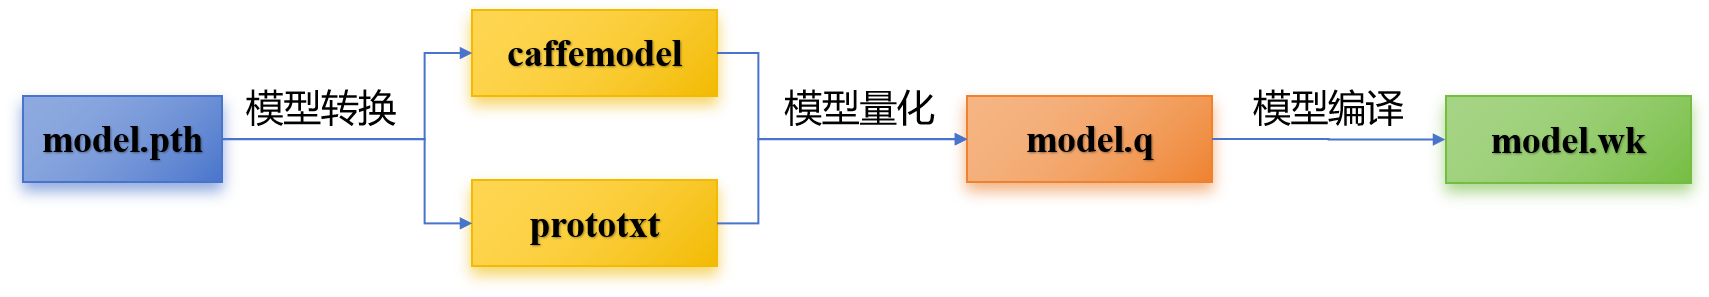
\includegraphics[width=14cm, height=3cm]{pic/pre-deploy.png}
    \caption{模型推理前置工作流程示意图}
    \label{pre-deploy}
\end{figure}

\subsection{模型推理}
在模型推理阶段,将本文提出的检测模型部署在海思Hi3516DV300边缘芯片平台,并基于摄像头sensor实时采集视频,转换为帧图像后,送入IVE、NNIE等智能计算平台进行模型推理,并经过CPU后处理,在显示屏上实时显示推理结果。

\textbf{(1)视频采集与裂缝实时检测}

海思Hi3516DV300平台实现裂缝实时检测的全流程图,如下图所示:

\begin{figure}[H]
    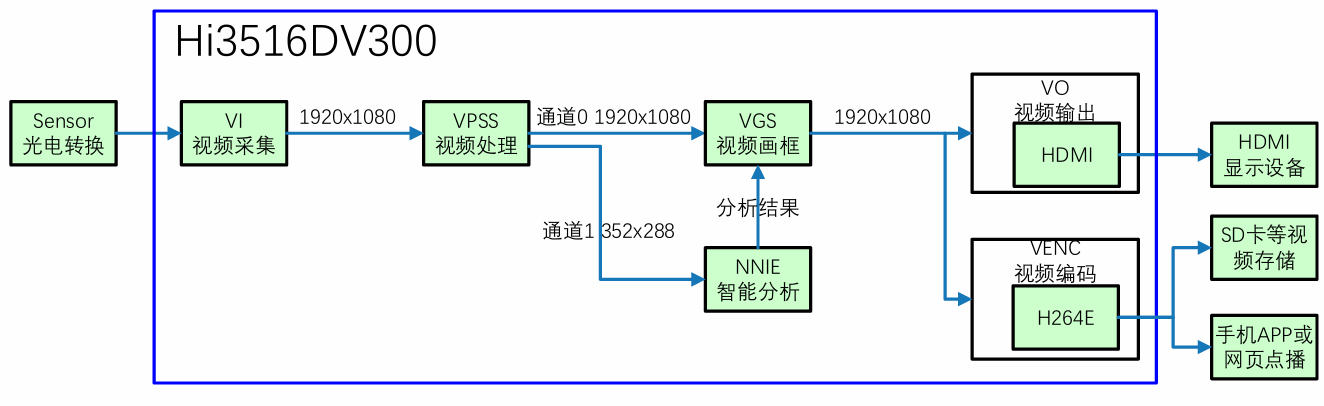
\includegraphics[width=14cm]{pic/detect-flow.png}
    \caption{裂缝实时检测流程示意图}
    \label{detect-flow}
\end{figure}

其中,VI是视频输入子系统,用于实时采集视频图像;
VPSS是视频处理子系统,用于实时处理采集的视频,以便用户获取视频帧,进行后续裂缝检测业务处理;
VO是视频输出模块,用于将处理后的视频帧,显示在屏幕设备上。

根据上图,VI为视频采集模块,采集图像送入VPSS进行视频处理,通道输出两路图像,通道0输出大分辨率图像用于输出显示,通道1输出小分辨率图像用于NNIE智能分析。
NNIE对裂缝图像推理完成后,VGS根据裂缝检测结果,在收到的通道0高分辨率图像上进行标注,再将标注后的图像送给VO模块显示。

\textbf{(2)NNIE智能计算与推理}

裂缝图像的检测任务,主要是在IVE、NNIE的智能计算平台完成的,CPU负责任务的调度和一些NNIE不支持的算子的运算。

首先从VPSS通道0获取$1920\times1080$的视频帧,再利用IVE智能视觉加速引擎,将该视频帧缩放到$480\times320$的尺寸大小(减小分辨率,从而加速推理)。
接着,将帧结构转换为IVE支持的图像数据结构,由IVE对图像进行色彩空间转换,将帧图像的YUV420SP格式图像,转换为裂缝检测模型支持的RGB三通道格式图像。
最后,送入NNIE,进行模型和任务推理。

待到推理任务完成后,由CPU对推理结果的张量进行后处理,得到每个像素点对应的类别索引。
再根据类别索引,将类别张量转换为RGB色彩的黑白图像数据结构。
最后,再由IVE换原图像色彩空间为YUV420SP格式,并送入VO模块显示。

其中,NNIE加速器进行模型推理的算法流程图,如下图所示:

\begin{figure}[H]
    \label{nnie-flow}
    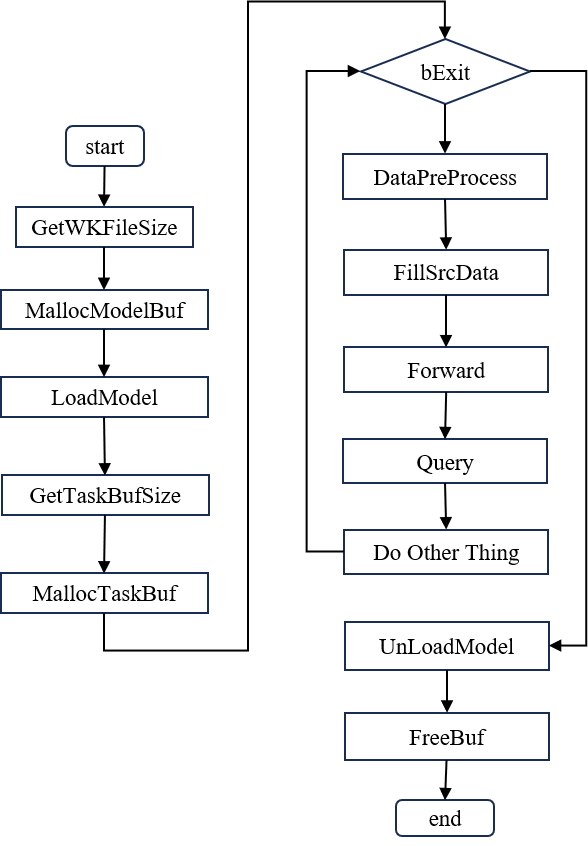
\includegraphics[width=8cm, height=10cm]{pic/nnie-flow-figure.png}
    \caption{NNIE模型推理流程图}
\end{figure}

根据上图,NNIE进行任务推理,具体包括以下步骤:

(1)CPU首先获取wk模型文件的大小,并为其分配内存,紧接着加载模型导内存中;

(2)然后,CPU会解析模型,获取模型执行推理任务时,数据所需的内存大小,并为其分配内存空间;

(3)模型加载和任务推理所需内存空间分配完成后,CPU会从VPSS通道0获取视频帧,并进行上文所述的图像格式等预处理过程;

(4)完成预处理后,会将图像数据填充到NNIE推理缓存区,并执行NNIE前向模型推理,并查询等待任务完成;

(5)任务完成后,开始下一帧图像的获取、预处理和推理任务。

裂缝检测任务结束后,CPU会卸载模型,并释放模型缓存和任务缓存的内存空间。

%————————————————————————————————————————————系统性能实验—————————————————————————————————————————————————————————————————————————

\section{系统性能测试及结果分析}

\subsection{模型量化前后精度误差}

模型量化,是将模型参数从32位的float型转换为8位的int型,会产生一定的精度损失。
但可以将模型大小减小为原来的1/4倍,从而节省内存、减小计算量,提高模型推理速度,降低系统检测时延。

\textbf{(1)余弦相似度}

余弦相似度指的是高维空间中两个向量的相似程度,其通过求两个向量的夹角余弦值,作为相似程度的量化标准。

余弦相似度计算公式如下:

\begin{equation}
    CS =  \frac{\mathbf{A} \cdot \mathbf{B}}{\|\mathbf{A}\|\|\mathbf{B}\|}  =  \frac{\sum_{i  = 1}^{n} A_{i} B_{i}}{\sqrt{\sum_{i = 1}^{n} A_{i}^{2}} \sqrt{\sum_{i =  1}^{n} B_{i}^{2}}}
\end{equation}

其中,$CS$表示相对余弦度,$\mathbf{A}$和$\mathbf{B}$分别是两个向量,$A_i$和$B_i$是向量中的对应分量,
$\mathbf{A} \cdot \mathbf{B}$表示向量的点积,
$\|\mathbf{A}\|$和$\|\mathbf{B}\|$分别是向量的欧几里得范数(即长度)。

相似余弦度在机器学习领域应用广泛,能有效评估文档或特征向量之间的相似性。

\textbf{(2)相对欧式距离}

相对欧式距离,RelativeEuclideanDistance,是通过将欧式距离归一化来衡量两个向量之间的距离,它能在一定程度上缓解尺度差异对距离度量的影响。

一般来说,计算相对欧式距离的方法是将两个向量之间的欧式距离除以向量长度的平均值,其计算公式如下:

\begin{equation}
    d_{rel}(A, B) = \frac{\sqrt{\sum_{i=1}^{n} (A_i - B_i)^2}}{f(A, B)} 
\end{equation}

其中,$d_{rel}(A, B)$表示向量$A$和$B$的相对欧式距离,$f(A, B)$是归一化因子,一般是向量长度的平均值。

\textbf{(3)量化前后精度误差}

对于模型量化前后推理结果,本文采用上述介绍的余弦相似度、相对欧式距离作为指标,衡量其误差大小和量化前后的精度损失。

随机选取测试集中的4张裂缝图片,输入模型进行推理,分别获取量化前后模型的输出结果,并计算两者之间的余弦相似度,
结果如下表\ref{}所示:

\begin{table}[H]
    \scriptsize
    \caption{模型量化前后精度误差}
    \label{quantification}
    \begin{tabular}{>{\centering\arraybackslash}p{4cm}>{\centering\arraybackslash}p{4cm}>{\centering\arraybackslash}p{4cm}}
    \toprule
     图片序号  & 余弦相似度 & 相对欧式距离\\ 
    \midrule
    \ding{172} & 0.999793  & 0.025967 \\
    \ding{173} & 0.999764  & 0.028165 \\ 
    \ding{174} & 0.999835  & 0.025581 \\ 
    \ding{175} & 0.999940  & 0.020071 \\ 
    \bottomrule
    \end{tabular}
\end{table}

根据上表可知,模型量化前后的推理结果之间余弦相似度超过0.99,相对欧式距离接近0.02,
精度损失很小,模型量化可行。

\subsection{系统功能测试}

系统功能测试效果,如下图\ref{func-test}。
其中红色像素表示对裂缝位置和类别的分割效果。

\begin{figure}[H]
    \subfloat[]{
        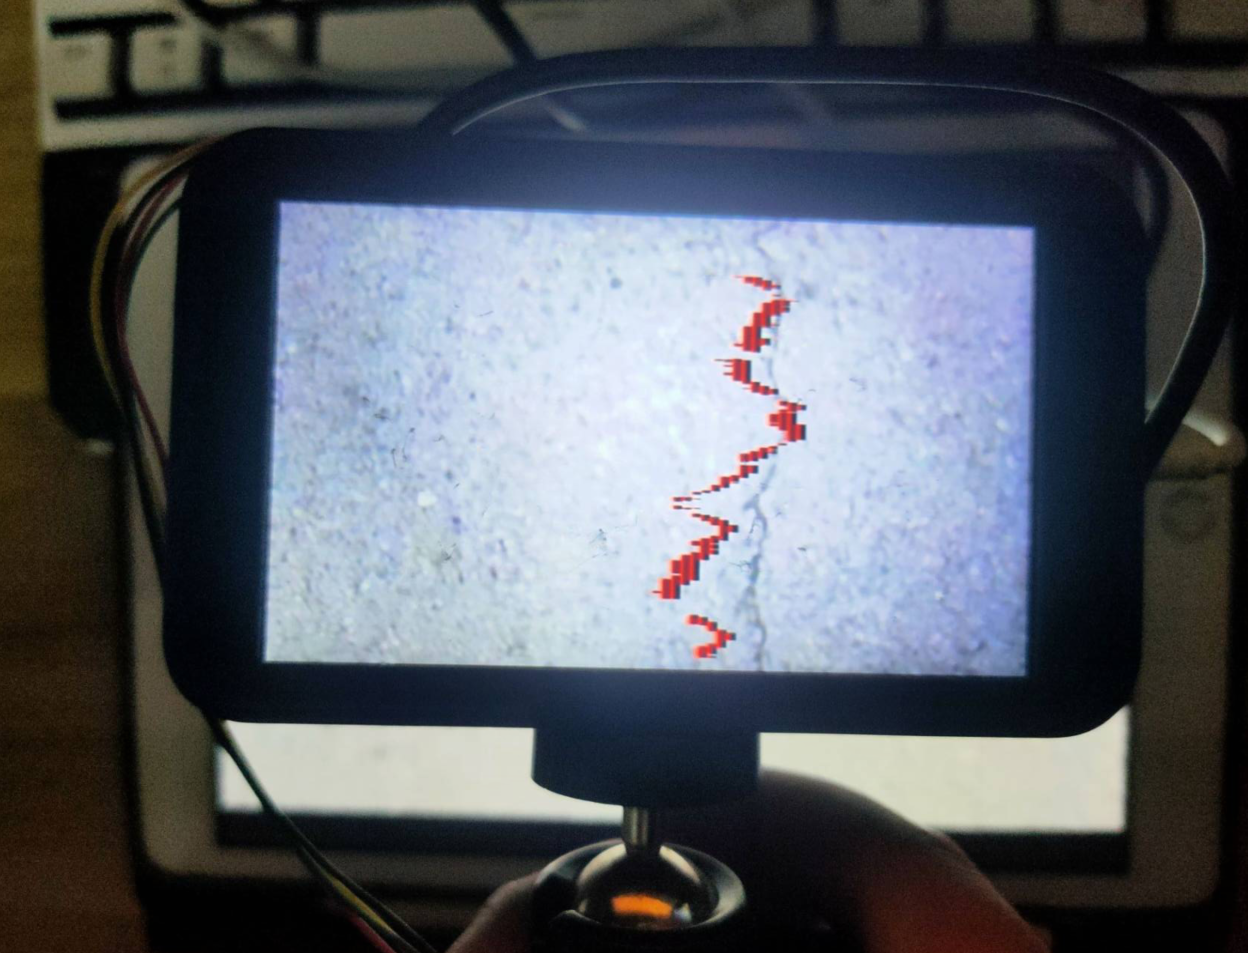
\includegraphics[width=7cm, height=5cm]{pic/func-test3.png}
        \label{func-test3}
    }
    \subfloat[]{
        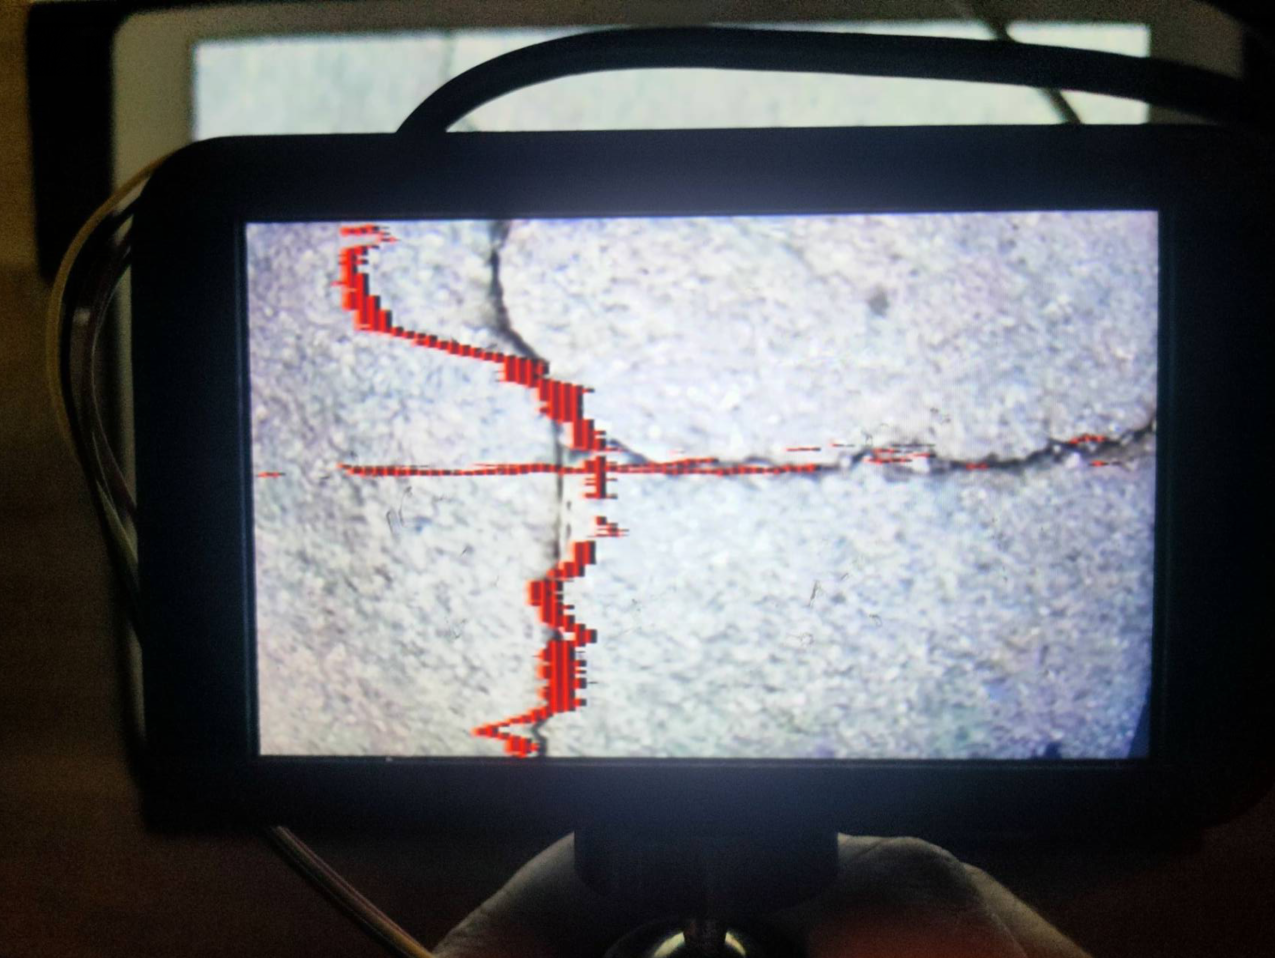
\includegraphics[width=7cm, height=5cm]{pic/func-test2.png}
        \label{func-test2}
    }
    \caption{系统功能测试示意图}
    \label{func-test}
\end{figure}  

根据实际测试效果,系统功能正常,且单帧裂缝图像推理耗时约0.5秒,满足实际低成本、低功耗边缘设备裂缝检测的速度和时延需求,具备裂缝检测实际工程应用的可行性。

\section{本章小结}
本章基于前文训练完成的算法模型,完成了模型在实际边缘设备中的部署和实时推理,设计并实现了边缘智能裂缝检测系统。
首先,介绍了模型部署的边缘芯片平台海思Hi3516DV300,包括其具体算力等硬件参数和芯片架构。
尤其是该芯片的智能计算平台NNIE和IVE,其中NNIE是专用于模型推理的AI加速器,IVE是传统计算机视觉图像处理的加速引擎。
紧接着,完成了边缘设备的系统环境的配置和搭建,包括OpenHarmony系统的交叉编译、烧录和测试。
然后,详细介绍了模型部署和裂缝检测系统开发的全过程,包括模型的量化、部署、实时裂缝图像采集、实时推理等工作。
最后,给出了系统性能测试及结果分析,包括模型量化前后的精度误差和系统功能测试,展示了系统的实际裂缝检测效果。

系统测试实验表明,在低成本、低功耗、资源有限的边缘设备上部署裂缝检测算法,精度损失很小,推理速度较快,满足实际裂缝检测系统的速度和时延需求,具备实际工程应用的可行性。